\documentclass{article}
\usepackage[utf8]{inputenc}
\usepackage[polish]{babel}
\usepackage{graphicx}
\usepackage[T1]{fontenc}
\usepackage{wrapfig}
\usepackage{fancyhdr}
\usepackage{tabularx}
\usepackage{hyperref}




%\usepackage[a4paper,top=2cm,bottom=2cm,left=3cm,right=3cm,marginparwidth=1.75cm]{geometry}
\usepackage[includeheadfoot,
            left=1in,
            right=1in,
            top=1cm,
            bottom=1cm,
            headheight=1cm]{geometry}


\pagestyle{fancy}
\fancyhf{}
\renewcommand{\headrulewidth}{0pt}
\renewcommand{\footrulewidth}{0pt}

\fancypagestyle{firstpage}
{
    \fancyhead[L]       % <-----------------LEWA STRONA-----------------
        {

            \vspace{0.25cm}
            \textbf{\textit{Miłosz Grześkowiak}} \\
            {\textit{1 Rok Informatyka Stosowana i Systemy Pomiarowe}} \\
            {\textit{24 Marca 2025}} \\
        }


    \fancyhead[R]   % <---------------------PRAWA STRONA------------
        {

             \vspace{0.25cm}
             \textit{25 Marca 2025}  \\
             {Prowadząca: } \\
             {\textit{dr Sylwia Owczarek}} \\

        }
}
\begin{document}
\textbf{ }\\
\textbf{ }\\
\thispagestyle{firstpage}
\centering
\section*{Ćwiczenie nr. 9}
\subsection*{Temat: Wyznaczenie modułu Younga metodą jednostronnego rozciągania}
\textbf{ }\\
\textbf{ }\\
\textbf{ }\\
\textbf{ }\\
\begin{tabularx}{0.8\textwidth} {
  | >{\centering\arraybackslash}X |     % 1  }
  | >{\centering\arraybackslash}X |     % 2  }   LICZBA
  | >{\centering\arraybackslash}X |     % 3  }   KOLUMN
  | >{\centering\arraybackslash}X |}    % 4  }
 \hline


 %---------------------------OPIS-------------------------------
 \#
 & Początkowa długość drutu [cm]
 & Średnica drutu [mm]
 & Średnica wskazówki [mm]  \\
%---------------------------OPIS-------------------------------


\hline
\hline
%---------------------------DANE-------------------------------
\hline 1 & 94.5 & 0.83 & 0.94 \\
\hline 2 & 93.5 & 0.83 & 0.96 \\
\hline 3 & 93.8 & 0.82 & 0.95 \\
\hline 4 & 94.2 & 0.83 & 0.97 \\
\hline 5 & 94.2 & 0.82 & 0.97 \\
\hline średnia & 94.04 & 0.826 & 0.958 \\
\hline odch. stand. & 0.35 & 0.004 & 0.012 \\
%---------------------------DANE-------------------------------
\hline
\end{tabularx}

\textbf{ }\\
\textbf{ }\\
\textbf{ }\\


\raggedright
    {
        {Dokładność wartości z pomiaru 1} \\
        {$\Delta_1$= 0.1cm}\\
        \textbf{ }\\
        {Dokładność wartości z pomiaru 2} \\
        {$\Delta_2$= 0.01mm}\\
        \textbf{ }\\
        {Dokładność wartości z pomiaru 3} \\
        {$\Delta_3$= 0.01mm}\\
        \textbf{ }\\
    }

\textbf{ }\\
\textbf{ }\\
\textbf{ }\\
\textbf{ }\\
Długość przy obciążeniu prostującym 0.5kg = 32dz
\centering
\begin{tabularx}{0.8\textwidth} {
  | >{\centering\arraybackslash}X |     % 1  }
  | >{\centering\arraybackslash}X |     % 2  }   LICZBA
  | >{\centering\arraybackslash}X |}    % 4  }
 \hline


 %---------------------------OPIS-------------------------------
obciążenie [kg]
 & długość drutu (pomiary rosnąco) [dz.]
 & długość drutu (pomiary malejąco) [dz.] \\
%---------------------------OPIS-------------------------------


\hline
\hline
%---------------------------DANE-------------------------------
\hline 1 & 33 & 32 \\
\hline 2 & 34 & 33 \\
\hline 3 & 35 & 34 \\
\hline 4 & 36 & 35 \\
\hline 5 & 37 & 36 \\
\hline 6 & 38 & 38 \\
\hline 6.5 & 38 & 38 \\
%---------------------------DANE-------------------------------
\hline
\end{tabularx}

\textbf{ }\\
\textbf{ }\\
\textbf{ }\\


\raggedright
    {
        {Dokładność wartości z pomiaru} \\
        {$\Delta = 1dz \approx 0.083mm$}\\
        \textbf{ }\\
    }

\textbf{} \\
\textbf{} \\
\textbf{} \\

\centering

\begin{table}[h]
  \centering
  \begin{tabular}{|c|c|}
    \hline
    Obciążenie [N] & $\Delta L$ [mm] \\ \hline
    9.81  & 0.041  \\ \hline
    19.62  & 0.127  \\ \hline
    29.43  & 0.207  \\ \hline
    39.24  & 0.290  \\ \hline
    49.05  & 0.373  \\ \hline
    58.86  & 0.498  \\ \hline
    63.76  & 0.498  \\ \hline
  \end{tabular}
\end{table}


\pagebreak


\centering

\section*{ZAGADNIENIA TEORETYCZNE}

{
\subsection*{Wprowadzenie}
Moduł Younga ($E$) jest jednym z podstawowych parametrów charakteryzujących właściwości mechaniczne materiałów. Określa on zależność między naprężeniem a odkształceniem w zakresie sprężystości, zgodnie z prawem Hooke'a. Wyznaczenie modułu Younga jest istotne w inżynierii materiałowej, konstrukcji maszyn oraz budownictwie, ponieważ pozwala ocenić sztywność materiału i jego odporność na odkształcenia pod wpływem sił zewnętrznych \cite{nowicki}.

\subsection*{Podstawy teoretyczne}
\subsubsection*{Prawo Hooke'a dla rozciągania}
Dla małych odkształceń, w zakresie sprężystości, naprężenie ($\sigma$) jest wprost proporcjonalne do odkształcenia względnego ($\varepsilon$):

\begin{equation}
    \sigma = E \cdot \varepsilon
\end{equation}

gdzie:
\begin{itemize}
    \item $\sigma$ - naprężenie mechaniczne [Pa],
    \item $E$ - moduł Younga [Pa],
    \item $\varepsilon$ - odkształcenie względne (bezwymiarowe).
\end{itemize}

\subsubsection*{Definicje naprężenia i odkształcenia}
\begin{itemize}
    \item \textbf{Naprężenie} ($\sigma$) - stosunek siły rozciągającej ($F$) do pola przekroju poprzecznego próbki ($S$):

    \begin{equation}
        \sigma = \frac{F}{S}
    \end{equation}

    \item \textbf{Odkształcenie względne} ($\varepsilon$) - stosunek przyrostu długości ($\Delta L$) do początkowej długości próbki ($L_0$):

    \begin{equation}
        \varepsilon = \frac{\Delta L}{L_0}
    \end{equation}
\end{itemize}

\subsubsection*{Zależność siły od wydłużenia}
Łącząc powyższe zależności, otrzymujemy wyrażenie na moduł Younga:

\begin{equation}
    E = \frac{\sigma}{\varepsilon} = \frac{F \cdot L_0}{S \cdot \Delta L}
\end{equation}

\subsection*{Metoda jednostronnego rozciągania}
W doświadczeniu wyznacza się moduł Younga poprzez pomiar wydłużenia próbki pod wpływem przyłożonej siły rozciągającej. Wykonuje się następujące kroki \cite{banasik}:

\begin{enumerate}
    \item \textbf{Przygotowanie próbki} - drut o znanych wymiarach (długość $L_0$, pole przekroju $S$).
    \item \textbf{Pomiar siły} - obciążenie próbki kolejnymi ciężarkami i rejestracja przyrostu długości ($\Delta L$).
    \item \textbf{Analiza danych} - sporządzenie wykresu zależności $F(\Delta L)$, który powinien być liniowy w zakresie sprężystości. Nachylenie prostej pozwala wyznaczyć $E$ po przekształceniu wzoru:

    \begin{equation}
        E = \frac{L_0}{S} \cdot \frac{\Delta F}{\Delta (\Delta L)}
    \end{equation}
\end{enumerate}

\subsection*{Czynniki wpływające na dokładność pomiaru}
\begin{itemize}
    \item Jednorodność materiału próbki,
    \item precyzja pomiaru długości i przekroju,
    \item zakres odkształceń sprężystych (aby uniknąć plastyczności),
    \item temperatura otoczenia (moduł Younga może zależeć od temperatury) \cite{szczeniowski}.
\end{itemize}

\subsection*{Podsumowanie}
Metoda jednostronnego rozciągania pozwala wyznaczyć moduł Younga w prosty sposób, opierając się na fundamentalnych zasadach mechaniki ośrodków ciągłych. Wynik doświadczenia zależy od dokładności pomiarów geometrycznych próbki oraz kontroli zakresu sprężystego materiału \cite{nowicki}.

\begin{thebibliography}{9}
\bibitem{nowicki}
Nowicki, B. (1998). \emph{Mechanika materiałów}. Warszawa: Wydawnictwo Naukowe PWN.

\bibitem{banasik}
Banasik, A. (2012). \emph{Wytrzymałość materiałów}. Kraków: Wydawnictwo Politechniki Krakowskiej.

\bibitem{szczeniowski}
Szczeniowski, S. (1980). \emph{Fizyka doświadczalna, cz. 1}. Warszawa: Państwowe Wydawnictwo Naukowe.

\bibitem{leyko}
Leyko, J. (2006). \emph{Mechanika ogólna}. Warszawa: Wydawnictwo Naukowe PWN.
\end{thebibliography}
}

\section*{OPIS DOŚWIADCZENIA}

{Doświadczenie polegało na obciążaniu drutu odważnikami, w celu ustalenia jak zmieniać się będzie jego długość. \\
Po obciążaniu druta, mierzone było położenie wskazówki przytwierdzonej do drutu.

}

\section*{OPRACOWANIE WYNIKÓW POMIARÓW}

{Moduł Younga możemy wyliczyć za pomocą współczynnika kierunkowego prostej regresji liniowej wyliczonej metodą najmniejszych kwadratów:
\[a = \frac{n\sum^n_{i=1}(x_iy_i) -\sum^n_{i=1}x_i\sum^n_{i=1}y_i}{n\sum^n_{i=1}x_i^2-(\sum^n_{i=1}x_i)^2}\]
\[b = \frac{\sum^n_{i=1}y_i-a\sum^n_{i=1}x_i}{n}\]

Korzystając z autorskiego skryptu w języku Python$^{[1]}$ obliczającego regresję liniową metodą najmniejszych kwadratów, wartości współczynników wynosiły odpowiednio \\
\textbf{} \\
$a = 109560.798$ i $b = 6.342$

\subsection*{Obliczenie modułu Younga za pomocą współczynnika kierunkowego prostej}
Moduł Younga możemy określić za pomocą współczynnika kierunkowego prostej. W tym wypadku współczynnik kierunkowy $a$ będzie równy współczynnikowi sprężystości $k$. \\
Współczynnik sprężystości jest równy:
\[k = \frac{F}{\Delta L}\]
Więc podstawiając do wzoru na moduł Younga, będzie on się prezentował następująco
\[E = \frac{k*L_0}{S}\]
Jedyną niewiadomą w tym wzorze pozostaje $S$, czyli pole przekroju poprzecznego drutu. Możemy je wyliczyć:
\[S = \pi*(\frac{\Phi}{2})^2=\pi*(\frac{0.000826m}{2})^2\approx5.36*10^{-7}m\]
Podstawiając wartości do wzoru:
\[E = \frac{109560\frac{N}{m}*0.9404m}{5.36*10^{-7}m}\approx192.221*10^{9}=192.221 GPa\]

\subsection*{Niepewność współczynnika kierunkowego regresji prostej}
Niepewność współczynnika kierunkowego możemy obliczyć ze wzoru
\[u(a) = \sqrt{\frac{\frac{1}{n-2}\sum^n_{i=1}(y_i-(ax_i+b))^2}{\sum^n_{i=1}(x-\bar x)^2}}\]
Korzystając ze skryptu w języku Python$^{[1]}$, wynik niepewności współczynnika kierunkowego wynosi $u(a) = 4.264379$. \\

\subsection*{Niepewność modułu Younga}
Niepewność modułu Younga możemy wyznaczyć ze wzoru
\[\Delta E = E\sqrt{(\frac{\Delta k}{k})^2+(\frac{\Delta_1 L}{L})^2+(\frac{\Delta S}{S})^2}\]
Gdzie:
\begin{itemize}
    \item $\Delta k = u(a)$
    \item $\Delta_1 L$ - niepewność przyrządu pomiarowego ($0.01mm=0.00001m$)
    \item $\Delta S = S\Delta d = \pi*d*\Delta d \approx 5.36*10^{-12}$ ($\Delta d$ - niepewność przyrządu pomiarowego)
\end{itemize}
Podstawiając wartości do wzoru
\[\Delta E = 192.221GPa\sqrt{(\frac{4.264379}{109.560\frac{N}{m}})^2+(\frac{0.00001}{0.9404m})^2+(\frac{5.36*10^{-12}}{5.36*10^{-7}m})^2}\approx7.481\]
Co oznacza, że
\[E = 192.221\pm 7.481GPa\]

\subsection*{Analiza wykresu}
Na podstawie zamieszczonego na ostatniej stronie sprawozdania wykresu (z którego określona została wartość współczynnika kierunkowego prostej regresji liniowej) można zauważyć, że punkty są bardzo zbliżone do prostej regresji, co wskazuje na to, że na pomiar nie wpływały żadne większe błędy pomiarowe.
}\\


\section*{WNIOSKI}

{Analizując wyniki, można dojść do wniosku, że pomiary zostały wykonane prawidłowo, z bardzo niskimi odchyleniami. \\
Na podstawie wartości modułu Younga, która wynosi $E = 192.221\pm 7.481GPa$ można określić materiał z jakiego został wykonany drut. \\
Biorąc pod uwagę dane na temat wartości modułu Younga dla wybranych materiałów$^{[2]}$ można określić, że materiał, z jakiego został wykonany drut to \textbf{stal niklowa}, \textbf{stal konstrukcyjna} lub \textbf{żelazo kute}.

\subsection*{Przypisy}
\begin{enumerate}
    \item \href{https://github.com/milosz0542/I-Pracownia-Fizyczna}{https://github.com/milosz0542/I-Pracownia-Fizyczna}
    \begin{itemize}
        \item Regresja liniowa /pomocenaukowe/linearregression.py
        \item Wykresy oraz współczynnik prostej regresji liniowej /pomocenaukowe/sprawozdanie4.ipynb
    \end{itemize}
    \item \href{https://www.engineeringtoolbox.com/young-modulus-d\_417.html}{https://www.engineeringtoolbox.com/young-modulus-d\_417.html}
\end{enumerate}
}

\pagebreak
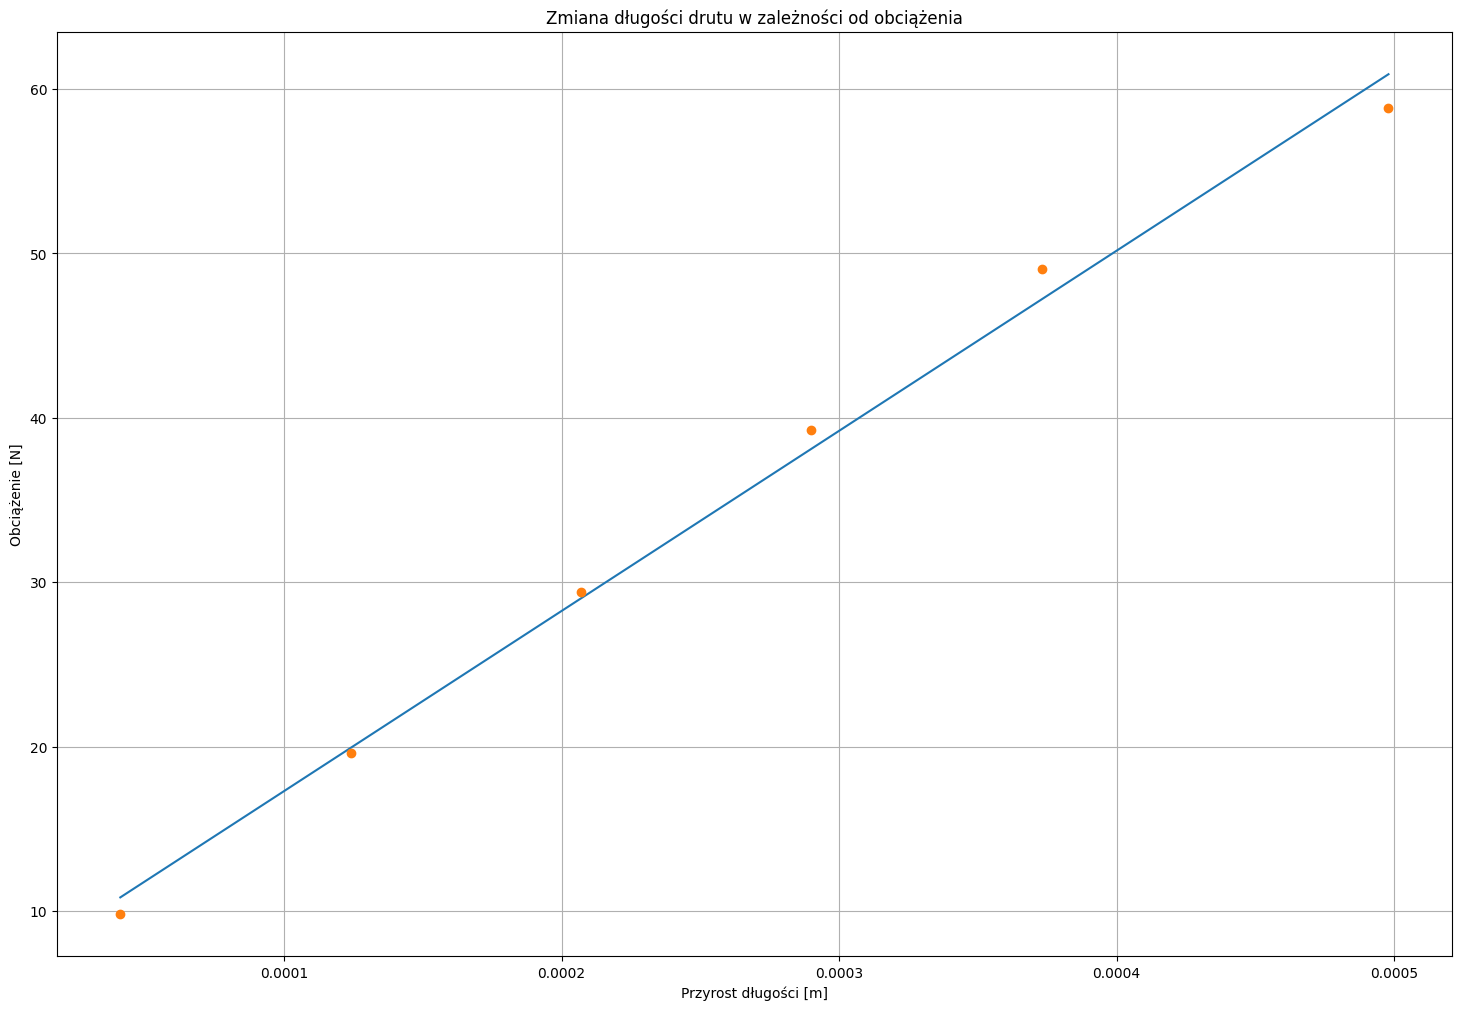
\includegraphics[angle=90, width=\textwidth, height=\textheight, keepaspectratio]{images/sprawozdanie4_1.png}
\end{document}


%Dodatkowe uwagi:

1. Sprawozdanie może być pisane ręcznie. Proszę jednak o czytelność pisma!!!

2. Sprawozdanie MUSI zawierać wszystkie części (tabela pomiarową, teoria,
przebieg ćwiczenia, obliczenia, niepewności, wnioski i wykresy). Brak
jakiejkolwiek części kwalifikuje do zwrotu złożonego sprawozdania bez dalszego
sprawdzania.

3. Wykresy należy zamieszczać na osobnych kartkach (format A4). Wykonywać za
pomocą komputera lub ręcznie na papierze milimetrowym. Należy tak dobrać
skalę, aby wykres zajmował całą stronę.

4. Punktów pomiarowych naniesionych na wykresach nie łączymy! W przypadku
dopasowania prostej regresji, wraz punktami na wykresie należy nanieść prostą
regresji.

5. Na wykresach razem z punktami należy nanieść niepewności pomiarowe w formie
tzw. krzyży niepewności pomiarowych.

6. Do sprawozdania należy dołączyć kartkę pomiarową z ćwiczenia podpisaną przez
prowadzącego.

7. Przy zapisie wyników wraz z niepewnością obowiązuje zasada podawania 2 cyfr
znaczących (instrukcja ONP).

8. Niepewności pomiarowe w większości przypadków wyliczamy bazując na trzech
metodach:
a) gdy mamy pomiary skorelowane korzystamy z zależności 17 w instrukcji ONP,
b) gdy mamy pomiary nieskorelowane korzystamy z zależności 15 w ONP,
c) w przypadku dopasowywania prostych regresji, niepewności obliczamy ze
wzorów 6 i 7 w ONP.